\documentclass[11pt,a4paper]{article}

% ── Typography & Layout ──────────────────────────────────────────────
\usepackage[T1]{fontenc}
\usepackage{lmodern}
\usepackage[utf8]{inputenc}
\usepackage[margin=1in]{geometry}
\usepackage{setspace}
\onehalfspacing
\usepackage{parskip}
\setlength{\parindent}{0pt}
\setlength{\parskip}{6pt plus 2pt minus 1pt}

% ── Colour Palette (Beige Theme) ─────────────────────────────────────
\usepackage{xcolor}
\definecolor{beigeback}{HTML}{F5F0E8}
\definecolor{beigedark}{HTML}{C9B99A}
\definecolor{beigemed}{HTML}{E0D6C8}
\definecolor{beigeaccent}{HTML}{8B7355}
\definecolor{beigetitle}{HTML}{5C4A32}
\definecolor{tablehead}{HTML}{E8DFD0}
\definecolor{darktext}{HTML}{3B3022}
\definecolor{rulecolor}{HTML}{A89880}

% ── Background ────────────────────────────────────────────────────────
\usepackage{background}
\SetBgColor{beigeback}
\SetBgOpacity{1.0}
\SetBgContents{}
\SetBgVshift{0pt}
\SetBgHshift{0pt}
\SetBgAngle{0}
\SetBgScale{1}

% ── Tables ────────────────────────────────────────────────────────────
\usepackage{booktabs}
\usepackage{tabularx}
\usepackage{array}
\usepackage{colortbl}
\usepackage{longtable}
\usepackage{multirow}
\newcolumntype{R}[1]{>{\raggedleft\arraybackslash}p{#1}}
\newcolumntype{L}[1]{>{\raggedright\arraybackslash}p{#1}}
\newcolumntype{C}[1]{>{\centering\arraybackslash}p{#1}}

% ── Graphics & Figures ────────────────────────────────────────────────
\usepackage{graphicx}
\usepackage{float}
\usepackage{caption}
\captionsetup{font=small,labelfont={bf,color=beigeaccent},labelsep=period,
              skip=6pt,belowskip=4pt}

% ── Headers & Footers ────────────────────────────────────────────────
\usepackage{fancyhdr}
\pagestyle{fancy}
\fancyhf{}
\fancyhead[L]{\small\color{beigeaccent}\textit{Artemis Track\,1 Research Report}}
\fancyhead[R]{\small\color{beigeaccent}\textit{Gupta \& Narayanan}}
\fancyfoot[C]{\color{beigeaccent}\thepage}
\renewcommand{\headrulewidth}{0.4pt}
\renewcommand{\headrule}{\hbox to\headwidth{\color{rulecolor}\leaders\hrule height \headrulewidth\hfill}}
\renewcommand{\footrulewidth}{0pt}

% ── Section Styling ───────────────────────────────────────────────────
\usepackage{titlesec}
\titleformat{\section}{\Large\bfseries\color{beigetitle}}{\thesection.}{0.75em}{}[\vspace{-2pt}{\color{rulecolor}\titlerule[0.6pt]}\vspace{4pt}]
\titleformat{\subsection}{\large\bfseries\color{beigeaccent}}{\thesubsection}{0.6em}{}
\titleformat{\subsubsection}{\normalsize\bfseries\color{beigeaccent}}{\thesubsubsection}{0.6em}{}
\titlespacing*{\section}{0pt}{18pt plus 4pt minus 2pt}{8pt plus 2pt minus 2pt}
\titlespacing*{\subsection}{0pt}{12pt plus 4pt minus 2pt}{6pt plus 2pt minus 2pt}

% ── Hyperlinks ────────────────────────────────────────────────────────
\usepackage{hyperref}
\hypersetup{colorlinks=true,linkcolor=beigeaccent,urlcolor=beigeaccent,citecolor=beigeaccent}

% ── Misc ──────────────────────────────────────────────────────────────
\usepackage{enumitem}
\setlist[itemize]{topsep=4pt,itemsep=2pt,leftmargin=1.2em}
\setlist[enumerate]{topsep=4pt,itemsep=2pt,leftmargin=1.2em}
\usepackage{textcomp}
\usepackage{amsmath}
\usepackage{amssymb}
\newcommand{\ieeecite}[1]{\hyperref[ref:#1]{[\ref*{ref:#1}]}}
\newcommand{\ieeecitetwo}[2]{\hyperref[ref:#1]{[\ref*{ref:#1}]}, \hyperref[ref:#2]{[\ref*{ref:#2}]}}
\newcommand{\ieeecitethree}[3]{\hyperref[ref:#1]{[\ref*{ref:#1}]}, \hyperref[ref:#2]{[\ref*{ref:#2}]}, \hyperref[ref:#3]{[\ref*{ref:#3}]}}

% ── Custom Environments ───────────────────────────────────────────────
\usepackage{tcolorbox}
\tcbuselibrary{skins}
\newtcolorbox{keyfinding}[1][]{%
  colback=beigemed!40,colframe=beigeaccent,fonttitle=\bfseries\color{beigetitle},
  boxrule=0.5pt,arc=2pt,left=6pt,right=6pt,top=4pt,bottom=4pt,#1}

\newtcolorbox{callout}[1][]{%
  colback=beigeback,colframe=beigedark,boxrule=0.4pt,arc=1.5pt,
  left=6pt,right=6pt,top=4pt,bottom=4pt,#1}

% ── Title ─────────────────────────────────────────────────────────────
\usepackage{epigraph}

\begin{document}
\begin{titlepage}

\begin{tikzpicture}[remember picture,overlay]
  \fill[beigedark] (current page.north west) rectangle ([yshift=-3.2cm]current page.north east);
  \node[anchor=center,yshift=-1.6cm] at (current page.north) {\Huge\bfseries\color{white} Artemis Track\,1};
  \node[anchor=center,yshift=-2.7cm] at (current page.north) {\large\color{white!90} Systematic Crypto Factor Rebalancing Strategy};
  \fill[beigetitle] ([yshift=-3.2cm]current page.north west) rectangle ([yshift=-3.35cm]current page.north east);
\end{tikzpicture}
\vspace{4cm}
\begin{center}
  {\LARGE\bfseries\color{beigetitle} Cross-Sectional Factor Portfolio\\[8pt] with Weekly Rebalancing}\\[24pt]
  {\large\color{beigeaccent} Shobhit Narayanan \quad$\cdot$\quad Aryan Gupta}\\[36pt]
  {\color{rulecolor}\rule{0.4\textwidth}{0.6pt}}\\[12pt]
  {\small\color{beigeaccent} Research Period: 2017--2026\\[3pt]
  In-Sample: 2021-05-10 \;\textendash\; 2024-11-11\\[3pt]
  Out-of-Sample: 2024-11-18 \;\textendash\; 2026-05-25\\[3pt]
  79\;weeks out-of-sample \;\textendash\; $\sim$113 Crypto Assets}
\end{center}
\vfill
\begin{center}
  {\footnotesize\color{beigeaccent} This report presents a systematic crypto factor rebalancing strategy for Track\,1 of the Artemis Quant Competition.\\[2pt]
  The goal is a rules-based portfolio with an economic rationale, statistical defensibility, and honest evaluation of limitations.}
\end{center}
\end{titlepage}

\newpage
\setcounter{page}{2}
\tableofcontents
\newpage

% ══════════════════════════════════════════════════════════════════════
\section{Executive Summary}
% ══════════════════════════════════════════════════════════════════════

This report presents a systematic crypto factor rebalancing strategy for Track\,1 of the Artemis Quant Competition.\footnote{A \emph{factor} is a measurable asset characteristic used to predict or explain cross-sectional returns. The concept is central to modern asset-pricing research.\ieeecitetwo{fama-french-1993}{carhart-1997}} The objective is to construct a rules-based portfolio that can be explained economically, tested statistically, and rebalanced on a \textbf{fixed weekly schedule}.\footnote{\emph{Out-of-sample} refers to a time period reserved for testing after all design choices have been made. This is the standard method for reducing overfitting risk, though a single holdout window remains a limited test.}

The core idea is simple: identify measurable characteristics of crypto assets that predict relative returns, combine them into a portfolio, and rebalance weekly. The implementation, however, requires careful attention to multiple-testing discipline, regime-aware risk sizing, and honest assessment of what the data actually supports versus what it merely suggests.

\begin{keyfinding}[title=Headline Result]
The \textbf{Sharpe Ensemble} achieves an out-of-sample Sharpe ratio of $+0.84$ (annualized return $+29.9\%$, volatility $35.8\%$, max drawdown $-24.7\%$) across 79\;weeks of held-out data from November 2024 to May 2026. Bitcoin returned $-12.3\%$ annualized over the same period, and the equal-weight market returned $-34.4\%$ annualized.
\end{keyfinding}

However, honest decomposition shows that this Sharpe ratio depends heavily on a single composite factor (MispricingM) and that the Priced Tilt sub-book is a net drag out-of-sample. The strategy is therefore best described as a \emph{single-factor portfolio with volatility and drawdown controls}, not a genuinely diversified multi-factor book. All limitations are discussed openly.

% ══════════════════════════════════════════════════════════════════════
\section{Glossary}
% ══════════════════════════════════════════════════════════════════════

\begin{longtable}{>{\bfseries\color{beigetitle}}p{2.8cm}p{9cm}p{2.4cm}}
\toprule
\rowcolor{tablehead}
Term & Definition & Key Reference \\
\midrule
\endfirsthead
\toprule
\rowcolor{tablehead}
Term & Definition & Key Reference \\
\midrule
\endhead
\bottomrule
\endlastfoot
Factor & A rule that ranks or tilts assets using a characteristic such as volatility, size, momentum, or drawdown & \ieeecitetwo{fama-french-1993}{han-2024} \\
Rebalancing & Periodically updating portfolio weights; this project rebalances weekly & \ieeecite{demiguel-2009} \\
IC & Information coefficient: the rank correlation between a factor score and next-period returns & \ieeecitetwo{spearman-1904}{grinold-kahn-2000} \\
Newey-West $t$ & A significance measure adjusted for autocorrelation and heteroskedasticity & \ieeecite{newey-west-1987} \\
ASD & Almost stochastic dominance: a distributional test suited to non-normal returns & \ieeecitetwo{leshno-levy-2002}{han-2024} \\
GX pricing & Giglio-Xiu latent-factor pricing: tests risk premia controlling for hidden common factors & \ieeecite{giglio-xiu-2021} \\
Sharpe ratio & Return per unit of volatility & \ieeecite{sharpe-1966} \\
Max drawdown & Largest peak-to-trough portfolio loss during the test window & \ieeecite{magdon-ismail-atiya-2004} \\
XGBoost & Gradient-boosted tree model used here to estimate regime probabilities & \ieeecite{chen-guestrin-2016} \\
Risk premium & Extra expected return for bearing systematic risk & \ieeecite{fama-french-1993} \\
Latent factor & A hidden common risk extracted statistically from returns & \ieeecite{giglio-xiu-2021} \\
Overfitting & Fitting historical noise rather than a repeatable relationship & \ieeecitetwo{chen-guestrin-2016}{brigida-2026} \\
Survivorship bias & Data problem where failed or delisted assets are missing from the historical universe & \ieeecitetwo{han-2024}{brigida-2026} \\
TVL & Total value locked: a DeFi usage metric, not a reliable standalone alpha signal & \ieeecitetwo{brigida-2025}{brigida-2026} \\
VolC & Volatility characteristic: a low-volatility crypto ranker & \ieeecite{frazzini-pedersen-2014} \\
MAXRET & Maximum recent return: a lottery-reversal signal & \ieeecitetwo{bali-2011}{han-2024} \\
RMOM & Risk-adjusted momentum: recent return scaled by recent volatility & \ieeecite{han-2024} \\
SMBC & Small-minus-big crypto size factor & \ieeecitetwo{fama-french-1993}{brigida-2026} \\
NetRel & Network-relative signal comparing a coin with related coins & \ieeecite{guo-2024} \\
CRASH8 & Rebound signal for deeply crashed coins & \ieeecite{han-2024} \\
BETA26 & High-beta crypto risk tilt & \ieeecitetwo{frazzini-pedersen-2014}{brigida-2026} \\
SKEW52 & Skewness or lottery-like payoff tilt & \ieeecite{bali-2011} \\
NEWC & Newer-coin seasoning tilt & \ieeecitetwo{han-2024}{brigida-2026} \\
\end{longtable}

\smallskip
The report uses \textbf{in-sample} to mean the research window used to study and build the model, and \textbf{out-of-sample} to mean the later window used to test whether the model remains effective after design choices have been finalized.

% ══════════════════════════════════════════════════════════════════════
\section{Competition Objective}
% ══════════════════════════════════════════════════════════════════════

Track\,1 asks for a systematic crypto factor rebalancing strategy. In practical terms, this means:

\begin{enumerate}[nosep]
  \item Define a tradable crypto universe.
  \item Build factor signals with a clear economic story.
  \item Rebalance the portfolio on a consistent weekly schedule.
  \item Evaluate returns, risk, turnover, drawdown, and robustness.
  \item Critically explain what could fail.
\end{enumerate}

The following sections address each requirement in turn, proceeding from data and universe construction through factor discovery and validation, strategy assembly, backtest results, and finally an honest critical evaluation.

% ══════════════════════════════════════════════════════════════════════
\section{Universe, Data, and Design Choices}
% ══════════════════════════════════════════════════════════════════════

The research uses a weekly crypto asset panel covering approximately 113 large-cap and upper-mid-cap cryptocurrency assets. The broad factor validation work spans 2017--2026, with the final strategy evaluated on a panel whose last 79\;weeks constitute the out-of-sample window ending on May\;25, 2026.

\begin{center}
\begin{tabular}{ll}
\toprule
\textbf{Split} & \textbf{Period} \\
\midrule
In-sample (main validation) & 2021-05-10 \;\textendash\; 2024-11-11 \\
Out-of-sample (main validation) & 2024-11-18 \;\textendash\; 2026-05-25 \\
\midrule
In-sample (final strategy) & Before 2024-11-25 \\
Out-of-sample (final strategy) & Final 79\;weeks \\
\bottomrule
\end{tabular}
\end{center}

The universe is drawn from CoinGecko market-capitalization rankings, with deliberate exclusions of stablecoins, wrapped duplicates, and bridged tokens. This universe occupies a specific economic niche that balances three competing considerations.

\subsection{Why This Universe?}

\textbf{Efficiency and coverage gaps.}\;
The largest crypto assets (top\;20 by market cap) are subject to intensive analyst coverage, institutional arbitrage via ETF flows, and deep on-chain surveillance. Cross-sectional factor premia in these names are likely compressed by the same mechanism that erodes anomalies in large-cap equities.\ieeecite{mclean-pontiff-2016} By extending into the upper-mid-cap tier (\#20--\#120), the universe captures assets where information asymmetry is structurally higher---fewer dedicated analysts, thinner institutional ownership, more heterogeneous investor bases---precisely the conditions under which behavioral mispricings persist.

\textbf{Execution feasibility.}\;
Extending below the top\;120 into micro-cap crypto introduces severe capacity constraints. Daily trading volumes below \$1\;M create market-impact costs exceeding 100\;bps per trade, rendering paper factor premia untradeable at any meaningful scale. The chosen universe ensures that most constituents trade above \$5\;M daily volume on major exchanges, keeping estimated one-way execution costs in the 10--30\;bps range for institutional-sized orders.

\textbf{Cross-sectional dispersion.}\;
Factor strategies require sufficient return dispersion across assets to generate meaningful long-short spreads. A universe restricted to the top\;10 assets offers too little variation in characteristics like size, volatility, and momentum. The ${\sim}113$-asset panel provides enough dispersion for quantile-sorted portfolios (top/bottom 30\%) to contain 15--20 assets per leg, ensuring adequate diversification within each portfolio tail.

\subsection{Validation Period and Dynamic Market Cap}

The primary validation window is anchored in May\;2021 to leverage a robust five-year data history while enforcing strict liquidity and survivorship controls. Assets are restricted to a minimum market capitalization of \$100\;M; any coin falling below this threshold is dynamically excluded from the following week's eligible list and its positions are immediately closed.

Crucially, this five-year timeline captures the profound post-COVID structural transformation of the crypto asset class. By training the strategy through the retail-driven speculative excess of 2021 and the systemic contagion of 2022, and validating it against the institutionalized, ETF-driven landscape of 2024--2026, we ensure that our factors demonstrate resilience across both historical liquidity crises and a permanently altered market structure.

The strategy excludes stablecoins, wrapped duplicates, and very low-quality assets wherever possible. Stablecoins lack the risk-return profile of volatile crypto assets. Wrapped assets duplicate exposures already present in the universe. Very illiquid assets produce paper profits that may not be tradable after accounting for slippage.

% ══════════════════════════════════════════════════════════════════════
\section{Factor Discovery and Validation Framework}
% ══════════════════════════════════════════════════════════════════════

The strategy begins with factor discovery. A factor is useful only if it passes at least one of three independent tests, each answering a different economic question. A factor does not need to pass all three: a 264-week crypto panel is too short to deliver $|t| \geq 2$ on every axis for every factor.

\subsection{Test\,1 --- Information Coefficient (IC)}

The information coefficient is the Spearman rank correlation between a factor's cross-sectional scores at week~$t$ and the realized returns at week~$t{+}1$. A positive direction-adjusted IC means the factor's bet ranked next-week winners above next-week losers. Typical useful ICs in crypto are small ($|\text{IC}| \approx 0.03$--$0.05$) because the asset class is noisy, but even small ICs compound into meaningful alpha when applied consistently across 50+ assets each week.

An important subtlety: some factors go \emph{long the bottom} of their characteristic sort. VolC, for example, buys low-volatility coins, so its raw IC against the volatility characteristic is \emph{negative}---which is the factor \emph{working}, not failing. All IC results are reported direction-raw; the sign should be read against the factor's intended bet direction. Statistical significance is assessed via Newey-West $t$-statistics with 4\;lags, which correct for the serial correlation and heteroskedasticity endemic in weekly crypto return series.\ieeecite{newey-west-1987}

\subsection{Test\,2 --- Almost Stochastic Dominance (ASD)}

The Sharpe ratio implicitly assumes normally distributed returns. Crypto factor returns are not: every factor in our panel rejects the Jarque-Bera normality test at the 5\% level, with excess kurtosis ranging from $+1.1$ to $+19.3$ and skewness from $-1.0$ to $+3.1$. Under these conditions, the Sharpe ratio understates tail risk and can rank strategies incorrectly.

Almost stochastic dominance avoids this by comparing entire return distributions without parametric assumptions.\ieeecite{leshno-levy-2002} The test produces two violation measures:

\begin{itemize}[nosep]
  \item $\varepsilon_1$ (AFSD): if $\varepsilon_1 \leq 5.9\%$, the factor \emph{almost first-order stochastically dominates} Bitcoin---meaning \emph{all} investors, regardless of risk preference, would prefer the factor's return distribution.
  \item $\varepsilon_2$ (ASSD): if $\varepsilon_2 \leq 3.2\%$, the factor \emph{almost second-order dominates} Bitcoin---meaning all \emph{risk-averse} investors would prefer it.
\end{itemize}

Recent crypto factor work applies this framework to cryptocurrency factor portfolios and demonstrates that several factors dominate benchmarks under ASD even when their Sharpe ratios are unremarkable, making ASD the appropriate test for fat-tailed crypto returns.\ieeecite{han-2024}

\subsection{Test\,3 --- Giglio-Xiu Latent-Factor Pricing (GX)}

The first two tests ask whether a factor \emph{works as a trading signal}. The Giglio-Xiu test asks a fundamentally different question: is the factor a \emph{priced source of systematic risk} in the cross-section? A factor is ``priced'' if assets that load more heavily on it earn systematically different expected returns---a risk premium, denoted~$\lambda$.\ieeecite{giglio-xiu-2021}

Three pricing methods are run side by side to triangulate the evidence:

\begin{enumerate}[nosep]
  \item \textbf{Fama-MacBeth (FMB)}: week-by-week cross-sectional regressions of returns on factor betas, averaging the estimated risk premia~$\lambda_t$ across weeks with Newey-West standard errors. This is the standard approach\ieeecite{fama-macbeth-1973} but is noisy when the number of factors approaches the number of assets per week.
  \item \textbf{GX observed-only}: a single cross-sectional regression on time-series average returns using heteroskedasticity-robust standard errors. More stable than FMB but ignores the possibility that omitted common risks contaminate the estimates.
  \item \textbf{GX full}: the most credible specification.\ieeecite{giglio-xiu-2021} After initial pricing, Bai-Ng information criteria select~$K$ hidden latent factors from the pricing residuals. Betas are then re-estimated on the combined observed~+ hidden factor set, and risk premia are re-priced. This removes contamination from unobserved systematic forces that would otherwise inflate or deflate the estimated~$\lambda$ for the observed factors.
\end{enumerate}

The GX-full $t$-statistic is the primary pricing metric reported throughout. A factor with $|t_{\text{gx}}| \geq 1.65$ is considered a statistically meaningful priced risk.

\subsection{From Tests to Portfolio Routes}

The three tests are not averaged into one score. They answer different questions, so they route factors to different jobs:

\begin{enumerate}[nosep]
  \item \textbf{Economic story required}: a factor needs a plausible mechanism before it is tested.
  \item \textbf{IC route}: factors with robust in-sample and out-of-sample ranking power become weekly rankers.
  \item \textbf{ASD route}: factors whose return distributions dominate Bitcoin become distributional mispricing candidates.
  \item \textbf{GX route}: factors that remain priced after observed and hidden risks are controlled for become priced-risk candidates.
  \item \textbf{Control route}: market, sparse-PCA, and macro-spanned directions are retained as pricing controls, not alpha trades.
\end{enumerate}

This is the central design choice. A weak IC does not automatically eliminate a factor, and a strong GX statistic does not automatically justify a large allocation. The test that a factor passes determines the job it is allowed to perform.

% ══════════════════════════════════════════════════════════════════════
\section{Factor Economics and Evidence}
% ══════════════════════════════════════════════════════════════════════

\subsection{The Economic Question}

Every factor starts with the same question: why would this trade pay? The answer cannot be ``because the backtest liked it.'' A factor is a repeated long--short trade, and the economic story determines both the direction of the trade and the test it should be judged by. The factors fall into five families.

\subsection{Classic Risk and Anomaly Factors}

\begin{center}
\small
\begin{tabularx}{\textwidth}{L{0.14\textwidth}L{0.25\textwidth}X}
\toprule
\rowcolor{tablehead}
\textbf{Factor} & \textbf{Trade} & \textbf{Why it might pay} \\
\midrule
RC & Hold the whole crypto market, value-weighted & This is the crypto market premium: compensation for bearing systematic crypto risk. It is not alpha because every long-only holder already earns it. We include RC so the other factors are measured net of market beta. \\
SMBC & Long small coins, short big coins & Small caps are less liquid, less covered, and riskier, so they should require extra expected return. This is the crypto version of the Fama--French SMB effect, though it can invert during ``flight to quality'' periods when capital crowds into BTC and ETH.\ieeecite{fama-french-1993} \\
MomC & Long 4-week winners, short losers & Investors can under-react to news, so recent winners may keep winning.\ieeecite{jegadeesh-titman-1993} In crypto, raw momentum also crashes violently when trends reverse. \\
VolC & Long calm coins, short volatile coins & Leverage-constrained and lottery-seeking investors can overpay for exciting high-volatility names, leaving lower-volatility coins cheap. This is the crypto analogue of betting against beta.\ieeecite{frazzini-pedersen-2014} \\
\bottomrule
\end{tabularx}
\end{center}

\subsection{Risk-Adjusted Momentum and Lottery Reversal}

Risk-adjusted momentum divides a recent trend by the coin's own recent volatility, which makes the signal closer to a short-horizon Sharpe ratio. The purpose is to strip out the noise that makes raw momentum unstable in crypto.

\begin{center}
\small
\begin{tabularx}{\textwidth}{L{0.16\textwidth}X}
\toprule
\rowcolor{tablehead}
\textbf{Factor} & \textbf{Trade} \\
\midrule
RMOM1w & Long coins with high 1-week return divided by 4-week volatility. \\
RMOM2w & Long coins with high 2-week return divided by 4-week volatility. \\
RMOM4w & Long coins with high 4-week return divided by 4-week volatility. \\
MAXRET & Rank by the highest single weekly return in the last 4 weeks. An extreme up-week is a lottery signal: if investors overpay for the jackpot coin, the correct trade is to fade the lottery.\ieeecitetwo{bali-2011}{han-2024} \\
\bottomrule
\end{tabularx}
\end{center}

\subsection{Fundamental Factors}

\begin{center}
\small
\begin{tabularx}{\textwidth}{L{0.14\textwidth}L{0.25\textwidth}X}
\toprule
\rowcolor{tablehead}
\textbf{Factor} & \textbf{Trade} & \textbf{Why it might pay} \\
\midrule
FunC & Long high fees-to-market-cap, short low & This is crypto value: protocols that generate real cash flow should be cheap relative to protocols that do not. The problem is coverage. Only about half the universe earns meaningful fees, so the factor is structurally under-powered. \\
TVLC & Long high TVL-to-market-cap, short low & This captures DeFi engagement per dollar of market value. The bull case is usage-backed value; the bear case is TVL irrelevance because the information is already priced. The sign is genuinely ambiguous before testing.\ieeecite{brigida-2025} \\
\bottomrule
\end{tabularx}
\end{center}

\subsection{Network and Structure Directions}

Network and structure factors need more unpacking because they are not all buy/sell signals. Some describe how crypto assets move in blocs. These directions are useful for diversification and for pricing controls, but many are not alpha trades.

\textbf{Coin networks.} A network is a set of dots connected by lines. Here each dot is a coin and each line means that two coins move together. We build the network from returns rather than drawing it by hand:

\begin{enumerate}[nosep]
  \item \textbf{Correlate every pair of coins.} On each rolling 12-week window, compute the Spearman rank correlation between every pair of coin returns. Spearman correlation is used because crypto has large outliers and rank correlation is less distorted by one extreme week.\ieeecite{spearman-1904}
  \item \textbf{Turn correlation into distance.} Distance is $\sqrt{2(1-\rho)}$. Correlation $+1$ becomes distance 0, while unrelated coins sit farther apart.
  \item \textbf{Keep the strongest skeleton.} A full graph connects every coin to every other coin and is too noisy. A minimum spanning tree keeps the smallest set of links needed to connect the universe, leaving the backbone of strongest relationships.
  \item \textbf{Find communities.} Louvain clustering groups the tree into communities where coins are more connected to each other than to outsiders. The clusters often resemble crypto narratives, but the algorithm only sees co-movement.
\end{enumerate}

Once clusters exist, two network factors follow naturally. NetMom is within-cluster momentum: inside each cluster, it compares each coin's 4-week momentum with its clustermates and backs the local leader against the laggard. NetRel is cross-cluster rotation: it compares each coin or cluster against the rest of the market and backs the narrative bloc pulling ahead of the others. This follows the broader idea that crypto returns contain asset-specific and network-like components.\ieeecitetwo{liu-tsyvinski-2021}{guo-2024}

\begin{figure}[H]
\centering
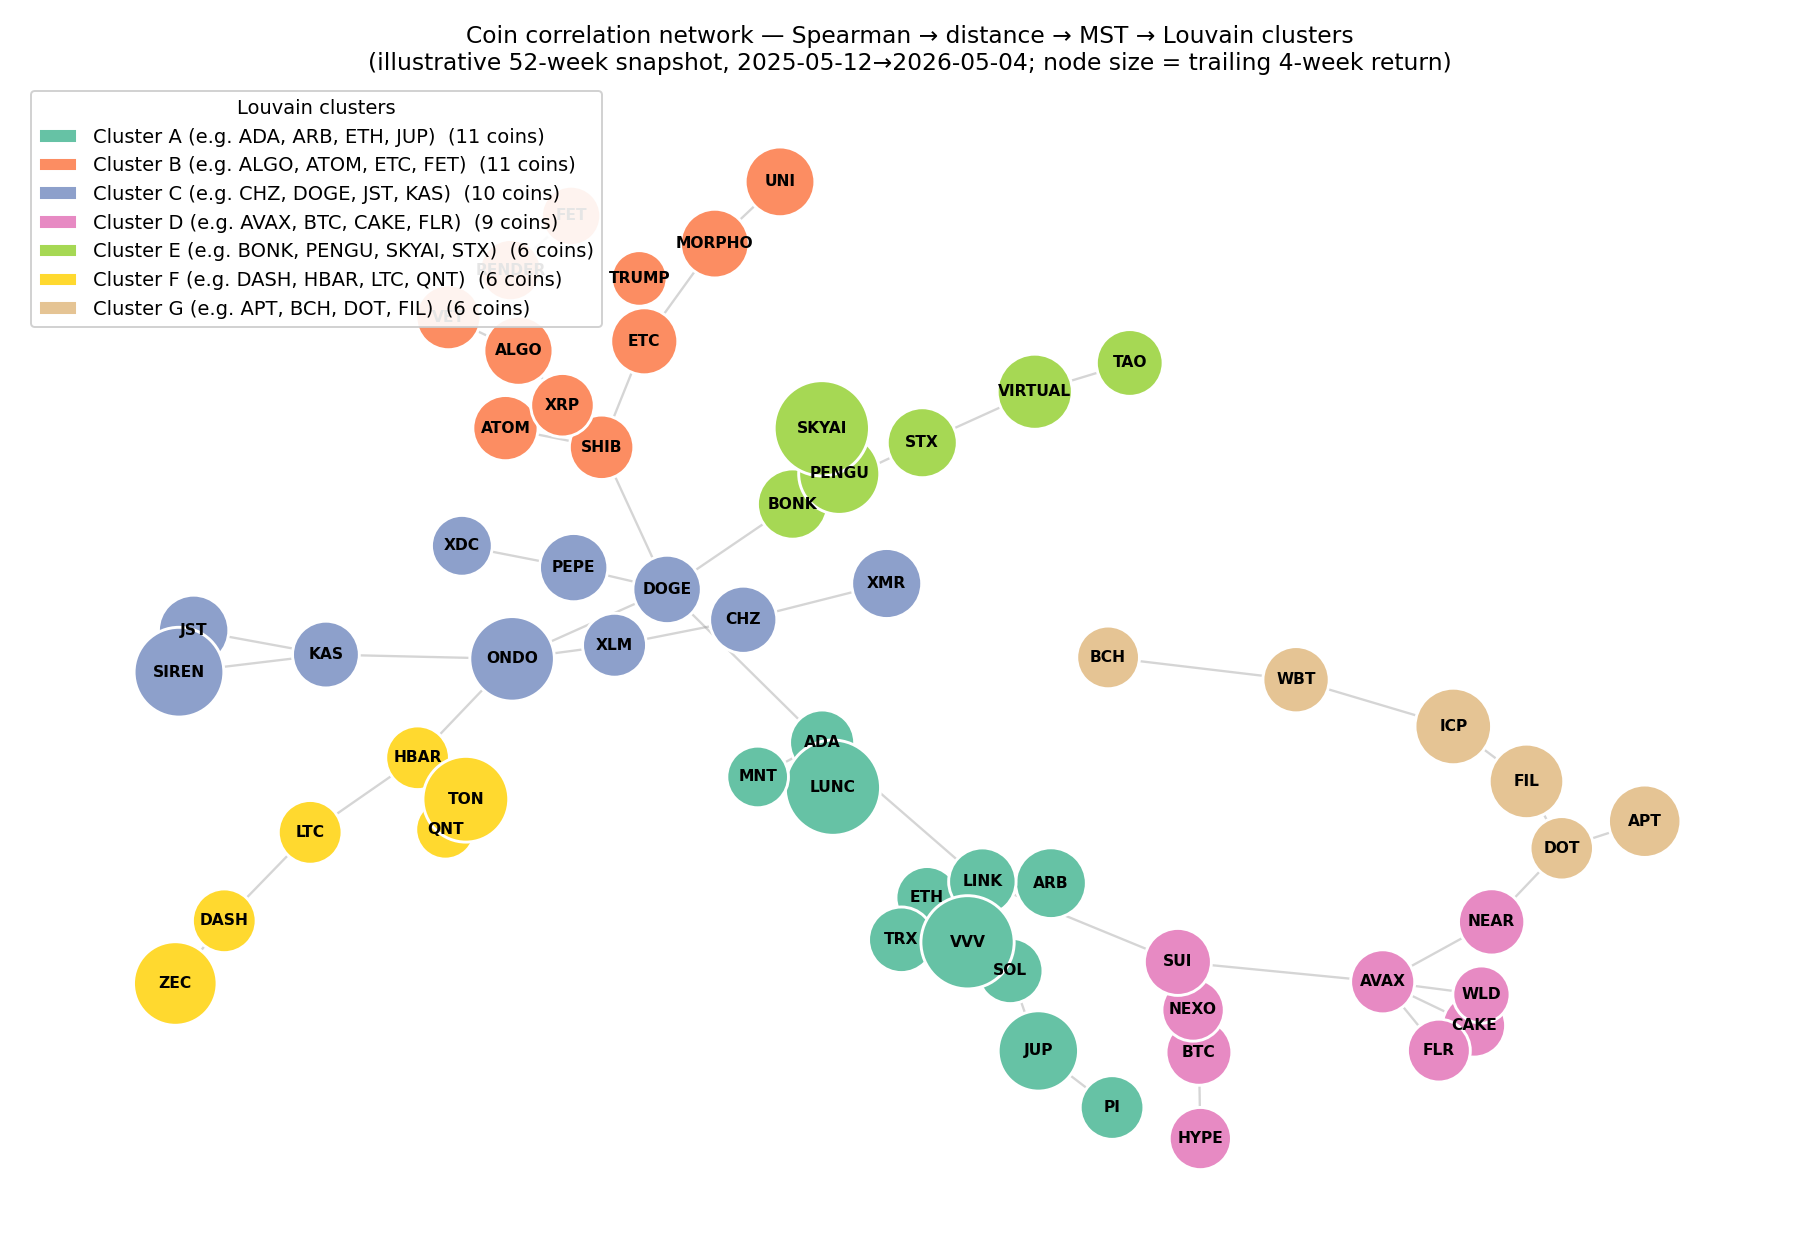
\includegraphics[width=\textwidth]{figures/network_clusters.png}
\caption{Coin correlation network with Louvain clusters. The graph is built from this project's own return panel using the Spearman correlation, distance transform, minimum spanning tree, and Louvain community detection pipeline. Each dot is a coin, each line is a strong retained co-movement link, and each colour is a data-driven cluster.}
\end{figure}

\begin{figure}[H]
\centering
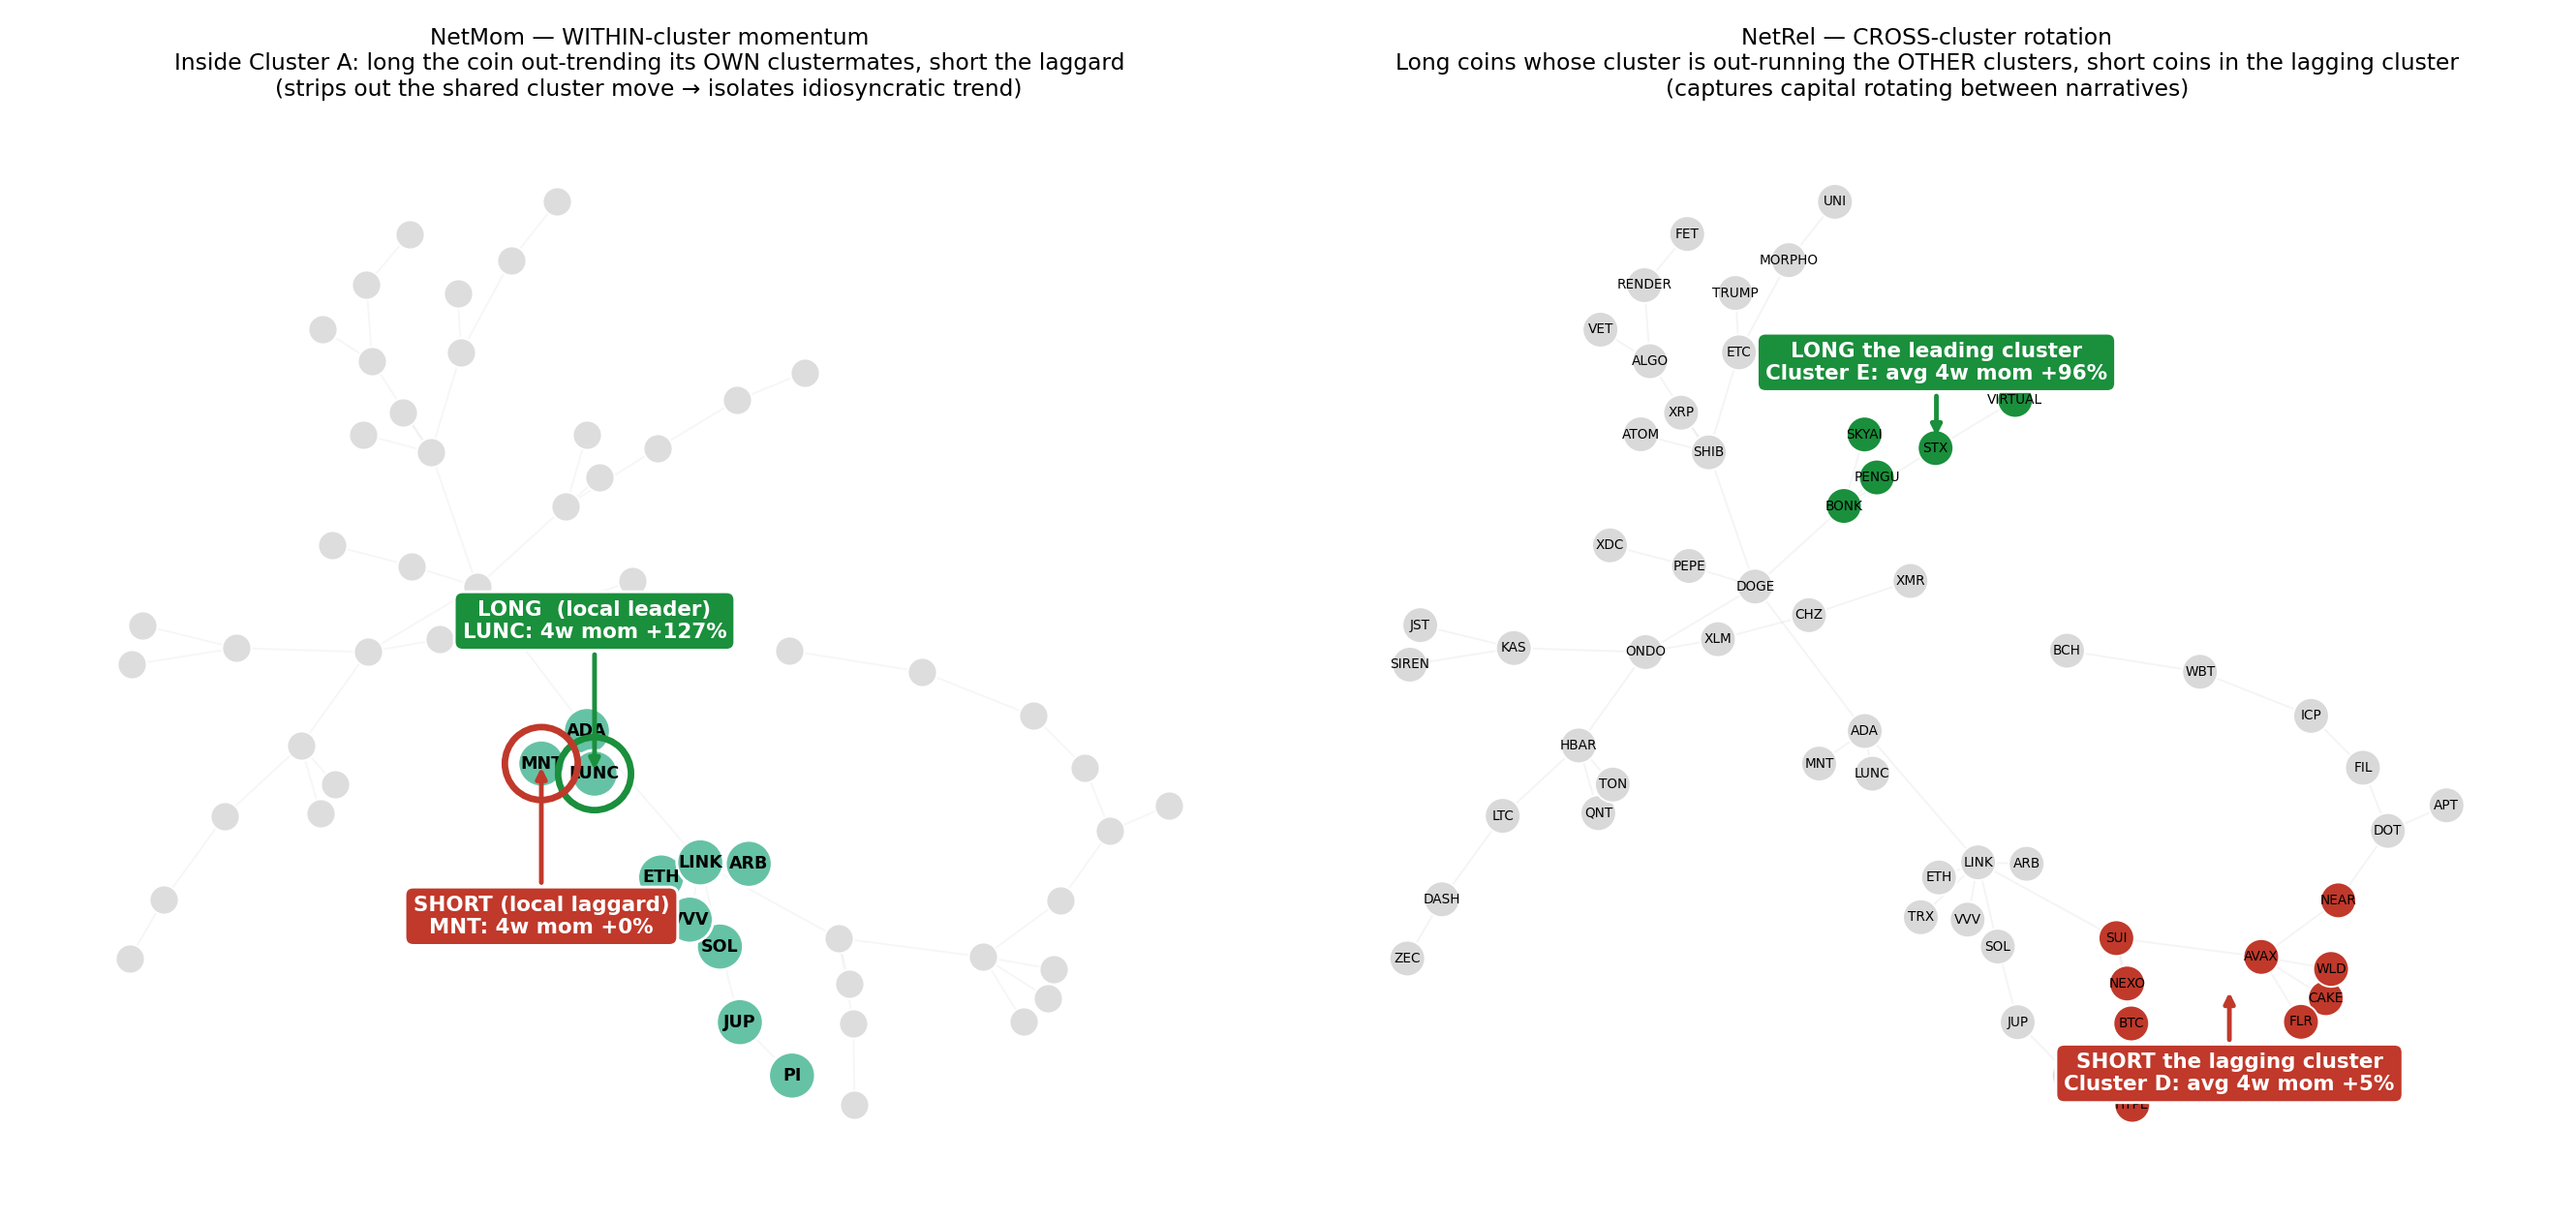
\includegraphics[width=\textwidth]{figures/netmom_netrel_schematic.png}
\caption{NetMom and NetRel illustrated on the same network. NetMom works inside one cluster by buying the local momentum leader and shorting the local laggard. NetRel works between clusters by buying coins in the leading narrative bloc and shorting coins in the lagging bloc. The figures are produced by \texttt{figures/make\_network\_viz.py}.}
\end{figure}

\textbf{Sparse PCA.} Ordinary PCA finds the main directions along which all coins move, but the resulting components load a little on many coins and are hard to interpret. Sparse PCA adds a penalty that pushes most loadings to zero, so each component loads on a smaller and more readable group. We extract four sparse components: SPC1 is a broad DeFi-majors or ``everything together'' direction; SPC2 is a payment and old-guard direction; SPC3 is an alt-L1 direction; and SPC4 is a legacy, privacy, and exchange-token direction. These are market-structure directions, not standalone trades.

\textbf{CCA.} Canonical correlation analysis asks how much of crypto is macro in disguise. One side contains the crypto return panel; the other contains BTC, SPX, DXY, UST10Y, and VIX. CCA finds the crypto-side combinations most correlated with macro-side combinations. CCA1--CCA3 therefore measure the slices of crypto that move with equity risk appetite, the dollar, rates, and volatility. They are controls, not alpha bets.

\begin{center}
\small
\begin{tabularx}{\textwidth}{L{0.16\textwidth}L{0.24\textwidth}X}
\toprule
\rowcolor{tablehead}
\textbf{Direction} & \textbf{What it represents} & \textbf{How to use it} \\
\midrule
NetMom & Within-cluster relative momentum & A coin-level signal: buy the local winner and short the local laggard inside the same narrative cluster. It removes the shared cluster move and tests idiosyncratic trend. \\
NetRel & Cross-cluster narrative rotation & A rotation signal: buy coins in clusters pulling ahead of the rest of crypto and short coins in lagging clusters. It captures capital moving between narratives. \\
SPC1--SPC4 & Sparse crypto-bloc directions & Risk controls: each component is a readable co-movement bloc such as broad market/DeFi-majors, payments, alt-L1s, or legacy/exchange exposure. \\
CCA1--CCA3 & Macro-spanned crypto directions & Macro controls: these measure the part of crypto that moves with BTC, equities, the dollar, rates, and volatility. They prevent macro beta from being mistaken for crypto alpha. \\
\bottomrule
\end{tabularx}
\end{center}
\smallskip
{\small Table\,4.\;Summary of network and structure directions.}

\subsection{Behavioral Factors}

The behavioral factor search tested 182 candidate specifications, then kept only factors that were economically interpretable, distinct from renamed VolC/MAXRET variants, and robust to multiple-testing correction.

\begin{center}
\small
\begin{tabularx}{\textwidth}{L{0.13\textwidth}L{0.30\textwidth}X}
\toprule
\rowcolor{tablehead}
\textbf{Factor} & \textbf{Trade} & \textbf{Investor behavior captured} \\
\midrule
NEWC & Long young coins, short seasoned coins & Newness or seasoning premium: investors demand compensation for holding less-proven assets. \\
SKEW52 & Long high 52-week skew, short low & Lottery memory: investors remember salient right-tail jumps and overpay for coins with upside histories. \\
CRASH8 & Long recently crashed coins, short resilient coins & Capitulation premium: freshly punished coins carry a priced rebound or crash-risk exposure. \\
BETA26 & Long high 26-week beta, short low & Speculative risk-on demand: high-beta coins are what investors reach for when they want amplified crypto exposure. \\
\bottomrule
\end{tabularx}
\end{center}

\subsection{Master Evidence Table}

The table below puts every factor through the same evidence lenses. IC $t$-statistics measure weekly ranking power; ASSD marks whether the factor return distribution is preferred to Bitcoin by risk-averse investors; GX reports the full Giglio--Xiu priced-risk test after observed and hidden factors are controlled for.\ieeecite{giglio-xiu-2021}

\begin{center}
\scriptsize
\setlength{\tabcolsep}{2.2pt}
\begin{longtable}{C{0.03\textwidth}L{0.095\textwidth}L{0.105\textwidth}L{0.22\textwidth}R{0.065\textwidth}R{0.07\textwidth}C{0.06\textwidth}R{0.08\textwidth}R{0.055\textwidth}L{0.12\textwidth}}
\toprule
\rowcolor{tablehead}
\textbf{\#} & \textbf{Factor} & \textbf{Family} & \textbf{Economic one-liner} & \textbf{IC IS $t$} & \textbf{IC OOS $t$} & \textbf{ASD} & \textbf{GX $\lambda$/yr} & \textbf{GX $t$} & \textbf{Grade} \\
\midrule
\endfirsthead
\toprule
\rowcolor{tablehead}
\textbf{\#} & \textbf{Factor} & \textbf{Family} & \textbf{Economic one-liner} & \textbf{IC IS $t$} & \textbf{IC OOS $t$} & \textbf{ASD} & \textbf{GX $\lambda$/yr} & \textbf{GX $t$} & \textbf{Grade} \\
\midrule
\endhead
1 & VolC & Anomaly & Low-vol beats high-vol & $-3.32$ & $-4.31$ & No & $-185.8\%$ & $-5.05$ & Confirmed \\
2 & MAXRET & Lottery & Short the lottery max-return signal & $-3.49$ & $-4.05$ & No & $+160.0\%$ & $+5.52$ & Confirmed \\
3 & CRASH8\textsuperscript{*} & Behavioral & Capitulation rebound & -- & -- & -- & $+177.9\%$ & $+4.79$ & Behavioral-confirmed \\
4 & BETA26\textsuperscript{*} & Behavioral & Speculative risk-on demand & -- & -- & -- & $+122.8\%$ & $+4.60$ & Behavioral-confirmed \\
5 & TVLC & Fundamental & DeFi engagement, TVL/mcap & -- & -- & -- & $-185.2\%$ & $-4.71$ & Priced risk \\
6 & RC & Market & Crypto market premium & -- & -- & -- & $+217.2\%$ & $+3.92$ & Priced risk \\
7 & SKEW52\textsuperscript{*} & Behavioral & Lottery memory, skew & -- & -- & -- & $+96.9\%$ & $+3.44$ & Behavioral-confirmed \\
8 & NEWC\textsuperscript{*} & Behavioral & Newness and seasoning & -- & -- & -- & $+114.1\%$ & $+3.43$ & Behavioral-confirmed \\
9 & RMOM1w & Risk-adj mom & 1-week Sharpe momentum & $-1.07$ & $-0.27$ & Yes & $+59.4\%$ & $+1.86$ & Priced risk \\
10 & SMBC & Anomaly & Size, small minus big & $+1.49$ & $+1.25$ & Yes & $+9.6\%$ & $+0.36$ & Suggestive \\
11 & NetRel & Structure & Cross-cluster rotation & $-1.72$ & $-0.10$ & Yes & $-0.2\%$ & $-0.01$ & Suggestive \\
12 & RMOM2w & Risk-adj mom & 2-week Sharpe momentum & $-2.46$ & $-0.24$ & Yes & $+31.3\%$ & $+1.05$ & Suggestive \\
13 & Mispricing\newline M & Composite & Equal-weight ASSD-dominant blend & -- & -- & Yes & -- & -- & Suggestive \\
14 & FunC & Fundamental & Fees/mcap value & -- & -- & -- & $+6.6\%$ & $+0.40$ & Economic-only \\
15 & RMOM4w & Risk-adj mom & 4-week Sharpe momentum & $-2.61$ & $-0.86$ & No & $+36.6\%$ & $+1.24$ & Not supported \\
16 & MomC & Anomaly & Raw 4-week momentum & $-1.66$ & $+0.13$ & No & $-3.3\%$ & $-0.10$ & Not supported \\
17 & NetMom & Structure & Within-cluster momentum & $-0.15$ & $-0.81$ & No & $+8.6\%$ & $+0.37$ & Not supported \\
18 & SPC3 & Structure & Alt-L1 bloc direction & -- & -- & No & $-221.4\%$ & $-3.88$ & Structure \\
19 & SPC1 & Structure & DeFi-majors bloc direction & -- & -- & No & $+57.6\%$ & $+1.08$ & Structure \\
20 & SPC2 & Structure & Payment/old-guard direction & -- & -- & No & $-56.0\%$ & $-1.47$ & Structure \\
21 & SPC4 & Structure & Legacy/exchange direction & -- & -- & No & $+93.5\%$ & $+1.42$ & Structure \\
22 & CCA1 & Structure & Macro-spanned direction 1 & -- & -- & -- & $-55.0\%$ & $-0.58$ & Structure \\
23 & CCA2 & Structure & Macro-spanned direction 2 & -- & -- & -- & $+6.6\%$ & $+0.58$ & Structure \\
24 & CCA3 & Structure & Macro-spanned direction 3 & -- & -- & -- & $+14.9\%$ & $+0.58$ & Structure \\
\bottomrule
\end{longtable}
\end{center}
\smallskip
{\small \textsuperscript{*}Behavioral factor priced jointly with $K_{\text{hidden}}=2$ hidden factors in the behavioral pricing run. Base factors use the full-sample GX-full pricing run.}

\subsection{How to Read the Grades}

\begin{center}
\small
\begin{tabularx}{\textwidth}{L{0.25\textwidth}X}
\toprule
\rowcolor{tablehead}
\textbf{Grade} & \textbf{Meaning} \\
\midrule
Confirmed & Strong on multiple independent lenses; defensible core signal. \\
Behavioral-confirmed & New behavioral factor that is strongly GX-priced and survives Bonferroni multiple-testing correction. \\
Priced risk & Compensated systematic exposure, but not necessarily a week-to-week trading edge. \\
Suggestive & Economic story remains intact with partial or semi-significant evidence. \\
Economic-only & Sound rationale, but this data cannot confirm it. \\
Structure & Risk direction describing how the market moves, not an alpha bet. \\
Not supported & Fails its own prediction on this sample. \\
\bottomrule
\end{tabularx}
\end{center}

The grading is deliberately not pass/fail. A 264-week crypto panel cannot hit $|t|\geq2$ everywhere, and a factor can be real on one lens while silent on another. VolC and MAXRET show the key nuance. Their weekly ranking evidence is strong: low-vol wins week to week, and lottery spikes reverse. But their long-run priced-premium evidence can point in the opposite direction from what a pure alpha-signal interpretation would suggest. The short-term ranking edge and the multi-year risk premium are not the same trade. That is why the strategy routes factors to different jobs instead of mechanically trading one master score.

\subsection{Factor Validation: Selected Exhibits}

The three charts below illustrate cumulative long-short returns and rolling IC significance for three representative factors spanning different roles in the strategy: VolC (confirmed weekly ranker), CRASH8 (behavioral priced-risk factor), and NetRel (structure/ASD route).

\begin{figure}[H]
\centering
\begin{minipage}[t]{0.485\textwidth}
  \centering
  
\includegraphics[width=\textwidth]{figures/volc_01_cumulative_return.png}
\end{minipage}\hfill
\begin{minipage}[t]{0.485\textwidth}
  \centering
  
\includegraphics[width=\textwidth]{figures/volc_02_rolling_ic_significance.png}
\end{minipage}
\caption{VolC (low-volatility anomaly). Left: cumulative long-short return with IS/OOS split. Right: rolling Newey-West IC $t$-statistic; values outside the $\pm1.65$ band indicate significant weekly ranking power.}
\end{figure}

\begin{figure}[H]
\centering
\begin{minipage}[t]{0.485\textwidth}
  \centering
  
\includegraphics[width=\textwidth]{figures/crash8_01_cumulative_return.png}
\end{minipage}\hfill
\begin{minipage}[t]{0.485\textwidth}
  \centering
  
\includegraphics[width=\textwidth]{figures/crash8_02_rolling_return_significance.png}
\end{minipage}
\caption{CRASH8 (capitulation rebound). Left: cumulative long-short return. Right: rolling return significance. CRASH8 is priced by the GX test ($t=+4.79$) rather than a consistent IC signal, so significance is episodic and concentrated around drawdown events.}
\end{figure}

\begin{figure}[H]
\centering
\begin{minipage}[t]{0.485\textwidth}
  \centering
  
\includegraphics[width=\textwidth]{figures/netrel_01_cumulative_return.png}
\end{minipage}\hfill
\begin{minipage}[t]{0.485\textwidth}
  \centering
  
\includegraphics[width=\textwidth]{figures/netrel_02_rolling_ic_significance.png}
\end{minipage}
\caption{NetRel (cross-cluster narrative rotation). Left: cumulative long-short return. Right: rolling IC significance. NetRel's IC is individually weak ($t=-0.10$ OOS) but its return distribution almost-stochastically dominates Bitcoin, justifying its role in the MispricingM composite rather than as a standalone ranker.}
\end{figure}

% ══════════════════════════════════════════════════════════════════════
\section{Final Strategy Construction}
% ══════════════════════════════════════════════════════════════════════

The key design choice in the final strategy construction is \emph{not} to blend every good-looking factor into one composite score. A single score is tempting because it is simple, but it erases the main lesson from Section\,5: factors are real in different ways. Some are weekly rankers, some are distributional mispricing edges, and some are priced systematic exposures. The final strategy therefore builds three separate sub-books, where each book groups factors that came out of the same exit of the factor router.

\subsection{From Router to Books}

\begin{figure}[H]
\centering
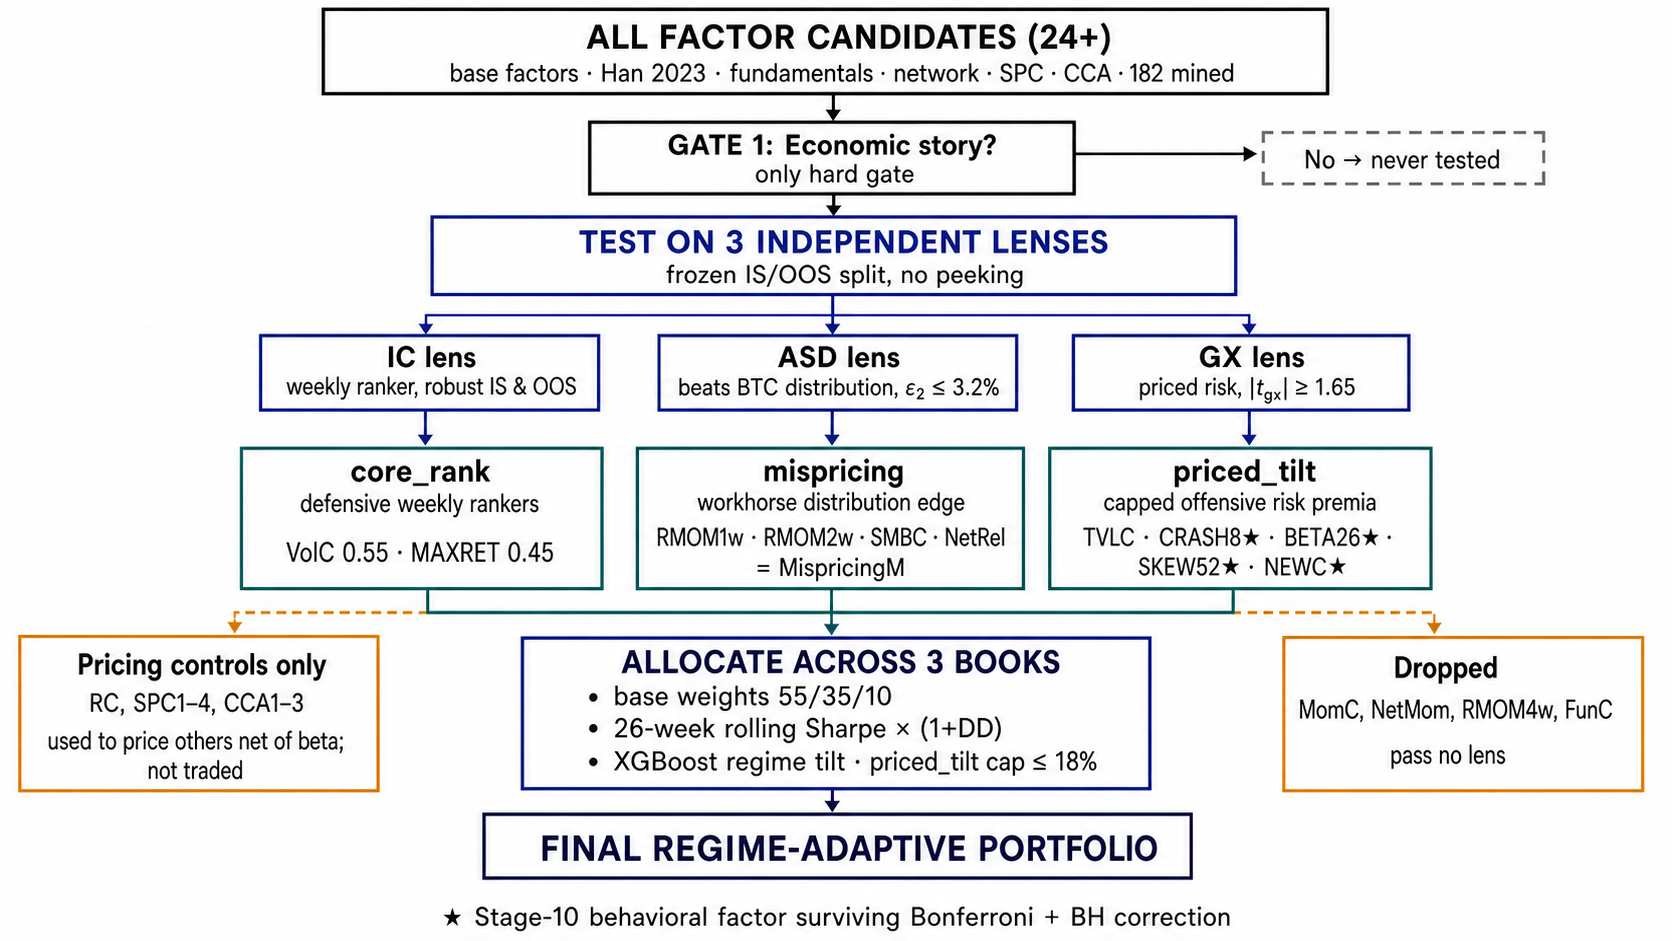
\includegraphics[width=\textwidth]{figures/factor_routing_graph.png}
\caption{Factor routing graph used to construct the three strategy books. The IC route becomes Core Rank, the ASD route becomes MispricingM, and the GX route becomes Priced Tilt. This preserves the kind of evidence each factor has instead of forcing all factors into one master score.}
\end{figure}

\begin{center}
\small
\begin{tabularx}{\textwidth}{L{0.15\textwidth}L{0.30\textwidth}L{0.25\textwidth}X}
\toprule
\rowcolor{tablehead}
\textbf{Sub-book} & \textbf{Members and weights} & \textbf{What unifies them} & \textbf{When it works} \\
\midrule
core\_rank & VolC 0.55; MAXRET 0.45 & Confirmed IC-robust weekly rankers. & Defensive sleeve for risk-off markets; low-volatility and lottery-fade act like flight-to-safety trades. \\
mispricing & RMOM1w, RMOM2w, SMBC, NetRel; 0.25 each & ASSD-dominant distribution edges; the MispricingM composite. & Workhorse alpha sleeve for normal markets; trimmed modestly in risk-off regimes. \\
priced\_tilt & TVLC 0.25; CRASH8 0.20; BETA26 0.20; SKEW52 0.20; NEWC 0.15 & Priced behavioral and DeFi systematic exposures. & Offensive sleeve for risk-on markets; capped because it is newest and most data-mined. \\
\bottomrule
\end{tabularx}
\end{center}
\smallskip
{\small Strategy sub-books and their economic roles.}

There are three reasons to keep these books separate rather than combine them into one signal.

\begin{enumerate}[nosep]
  \item \textbf{Factors of the same kind share a regime.} Weekly rankers work best when the market is defensive; priced and behavioral tilts are naturally more offensive. A monolithic score cannot lean toward the sleeve that matches the current market state.
  \item \textbf{Within-book averaging diversifies common noise.} The four mispricing sleeves are individually only Suggestive, but they share a common mispricing signal; averaging keeps the common signal and cancels idiosyncratic noise.\ieeecitetwo{stambaugh-yuan-2017}{han-2024} The behavioral sleeve is also designed to avoid putting all weight on one correlated effect.
  \item \textbf{Different books need different risk budgets.} A defensive ranker book can carry more gross exposure in a downturn; an offensive tilt book should be cut hard in the same environment. Separate books let each sleeve carry its own regime-dependent gross exposure.
\end{enumerate}

\subsection{Why MispricingM Becomes a Book}

The mispricing book is exactly the MispricingM composite developed in Section\,5: SMBC, NetRel, RMOM1w, and RMOM2w at equal weights. Individually, these factors are not clean weekly rankers. Together, they form the equal-weight blend that almost-stochastically dominates Bitcoin. The final strategy construction simply promotes that research prototype into a live sub-book.

\begin{center}
\small
\begin{tabular}{lccc}
\toprule
\rowcolor{tablehead}
\textbf{Window} & \textbf{Ann.\ return} & \textbf{Sharpe} & \textbf{$t$-stat} \\
\midrule
IS  & $+31.0\%$ & $+1.23$ & $+2.31$ \\
OOS & $+34.1\%$ & $+1.50$ & $+1.60$ \\
\bottomrule
\end{tabular}
\end{center}
\smallskip
{\small MispricingM performance by window.}

This is why NetRel reappears in the final strategy. It is not being smuggled back in after failing as a weekly ranker. It was routed here by the ASD lens in Section\,5, and this book is the trading home of that route.

The honesty flag is kept visible: factor selection for the mispricing book uses full-sample ASD, which technically sees the OOS window. To make that transparent, the validation pipeline re-reports $\varepsilon_2$ separately for IS, full sample, and OOS. The dominance is not only an OOS artifact, but the selection process is still not a perfectly untouched holdout.

\subsection{Why Priced Tilt Is Low-Correlation}

The priced\_tilt book is deliberately not one behavioral trade repeated under four names. The behavioral factors are chosen to be economically distinct and mostly low-correlation:

\begin{center}
\small
\begin{tabular}{lrrrr}
\toprule
\rowcolor{tablehead}
 & \textbf{NEWC} & \textbf{SKEW52} & \textbf{CRASH8} & \textbf{BETA26} \\
\midrule
NEWC   & $+1.00$ & $+0.03$ & $+0.63$ & $+0.10$ \\
SKEW52 & $+0.03$ & $+1.00$ & $+0.20$ & $+0.09$ \\
CRASH8 & $+0.63$ & $+0.20$ & $+1.00$ & $+0.17$ \\
BETA26 & $+0.10$ & $+0.09$ & $+0.17$ & $+1.00$ \\
\bottomrule
\end{tabular}
\end{center}
\smallskip
{\small Behavioral factor correlation matrix.}

Most pairs are close to zero. The one meaningful correlation, NEWC with CRASH8 at $+0.63$, is economically sensible because younger coins are more crash-prone. Both still survive jointly in the GX model, so the pair is not simply one trade wearing two labels. TVLC rides alongside these behavioral factors as the priced DeFi-engagement premium.

\subsection{Causal Allocation Across Books}

The book weights are adjusted dynamically each week. Each week, the allocation is set by a causal rule that uses only information available before that week:

\begin{enumerate}[nosep]
  \item \textbf{Start from a base allocation.} The Balanced variant starts at mispricing 55\%, core\_rank 35\%, and priced\_tilt 10\%. The Sharpe variant leans harder on the workhorse book, while the Defensive variant drops the offensive sleeve entirely.
  \item \textbf{Re-weight toward what has been working.} For each book, look back 26 weeks and score realized usefulness as $\max(\text{Sharpe},0)\times(1+\text{drawdown})$. A book that earns returns without drawing down receives more weight; a book that bleeds receives less.
  \item \textbf{Tilt by regime.} An XGBoost regime model outputs Risk-On, Neutral, and Risk-Off probabilities.\ieeecite{chen-guestrin-2016} Mispricing is nudged up in risk-on markets, core\_rank is nudged up in risk-off markets, and priced\_tilt is increased only when the regime supports risk-taking.
  \item \textbf{Cap the offensive sleeve.} priced\_tilt is hard-capped at 18\% of book allocation. It comes from a 182-candidate behavioral search, so it is never allowed to dominate the portfolio just because its recent run looks hot.
\end{enumerate}

\begin{center}
\small
\begin{tabular}{lccc}
\toprule
\rowcolor{tablehead}
\textbf{Variant} & \textbf{Mispricing} & \textbf{core\_rank} & \textbf{priced\_tilt} \\
\midrule
Sharpe & $92\%$ & $8\%$ & $0\%$ \\
Balanced & $55\%$ & $35\%$ & $10\%$ \\
Defensive & $65\%$ & $35\%$ & $0\%$ \\
\bottomrule
\end{tabular}
\end{center}
\smallskip
{\small Base allocations before rolling-performance and regime adjustments.}

\subsection{Regime Filtering and Final Weights}

The regime filter is a sizing layer, not a separate alpha model. Its job is to decide how much capital each book should receive after the base allocation and rolling-performance score have already been computed. This keeps the use of machine learning narrow: XGBoost estimates whether the market looks Risk-On, Neutral, or Risk-Off, and the allocator uses those probabilities to nudge book weights rather than to forecast individual coin returns.\ieeecite{chen-guestrin-2016}

This distinction matters because the available crypto return history is short and complex models overfit easily. The regime filter is therefore deliberately conservative. In Risk-Off states, core\_rank receives more weight because low-volatility and lottery-fade trades are defensive. In Risk-On states, mispricing can receive more weight and priced\_tilt is allowed to participate, subject to its hard cap. In Neutral states, the allocator stays closer to the blended base allocation.

\begin{center}
\small
\begin{tabular}{lccc}
\toprule
\rowcolor{tablehead}
\textbf{Variant} & \textbf{MispricingM} & \textbf{Core Rank} & \textbf{Priced Tilt} \\
\midrule
Sharpe Ensemble    & 80.8\% & 15.3\% & 3.9\% \\
Balanced Ensemble  & 54.8\% & 36.7\% & 8.5\% \\
Defensive Ensemble & 60.4\% & 35.7\% & 3.9\% \\
\bottomrule
\end{tabular}
\end{center}
\smallskip
{\small Realized average ensemble allocations after rolling-performance scoring, regime filtering, and caps.}

The realized weights show the constraint in action. Even the Sharpe Ensemble, which starts from a highly concentrated mispricing prior, still leaves a small allocation to Core Rank and keeps Priced Tilt below 4\%. Balanced Ensemble gives more capital to Core Rank and permits a larger but still capped Priced Tilt sleeve.

\begin{figure}[H]
\centering

\includegraphics[width=0.85\textwidth]{figures/image5.png}
\caption{Sharpe Ensemble allocation over time. The strategy gives most capital to MispricingM and keeps priced-risk exposure capped.}
\end{figure}

\begin{figure}[H]
\centering

\includegraphics[width=0.85\textwidth]{figures/image2.png}
\caption{Balanced Ensemble allocation over time. This variant gives more weight to Core Rank and is designed to reduce dependence on the mispricing sleeve.}
\end{figure}

% ══════════════════════════════════════════════════════════════════════
\section{Backtest Results}
% ══════════════════════════════════════════════════════════════════════

The full-window results show that the final ensembles reduce drawdown materially compared with Bitcoin and the equal-weight market, while still earning attractive returns.

\begin{center}
\small
\begin{tabular}{lcccccl}
\toprule
\rowcolor{tablehead}
\textbf{Strategy} & \textbf{Sharpe} & \textbf{Ann.\ return} & \textbf{Vol} & \textbf{Max DD} & \textbf{Hit rate} & \textbf{Weeks} \\
\midrule
SE  & $+1.27$ & $+64.7\%$ & $51.1\%$ & $-45.3\%$ & 53\% & 374 \\
BE  & $+1.18$ & $+51.1\%$ & $43.4\%$ & $-41.4\%$ & 54\% & 374 \\
DE  & $+1.21$ & $+54.4\%$ & $45.0\%$ & $-42.4\%$ & 53\% & 374 \\
MM  & $+1.24$ & $+76.5\%$ & $61.9\%$ & $-46.6\%$ & 54\% & 374 \\
CR  & $+0.53$ & $+18.5\%$ & $35.1\%$ & $-49.3\%$ & 49\% & 374 \\
PT  & $+0.30$ & $+11.1\%$ & $36.9\%$ & $-49.1\%$ & 47\% & 374 \\
EW  & $+0.82$ & $+65.7\%$ & $80.5\%$ & $-80.6\%$ & 55\% & 373 \\
BTC & $+0.92$ & $+54.4\%$ & $59.0\%$ & $-75.2\%$ & 52\% & 373 \\
\bottomrule
\end{tabular}
\end{center}
\smallskip
{\small Table\,8.\;Full-window performance (in-sample\;+\;out-of-sample). SE\;=\;Sharpe Ensemble, BE\;=\;Balanced Ensemble, DE\;=\;Defensive Ensemble, MM\;=\;MispricingM, CR\;=\;Core Rank, PT\;=\;Priced Tilt, EW\;=\;Equal-Weight Market, BTC\;=\;Bitcoin.}

\begin{center}
\small
\begin{tabular}{lcccccl}
\toprule
\rowcolor{tablehead}
\textbf{Strategy} & \textbf{Sharpe} & \textbf{Ann.\ return} & \textbf{Vol} & \textbf{Max DD} & \textbf{Hit rate} & \textbf{Weeks} \\
\midrule
SE  & $+1.36$ & $+74.0\%$ & $54.4\%$ & $-45.3\%$ & 54\% & 295 \\
BE  & $+1.28$ & $+59.7\%$ & $46.7\%$ & $-41.4\%$ & 55\% & 295 \\
DE  & $+1.31$ & $+63.2\%$ & $48.4\%$ & $-42.4\%$ & 53\% & 295 \\
EW  & $+1.10$ & $+92.1\%$ & $83.4\%$ & $-80.6\%$ & 58\% & 295 \\
BTC & $+1.14$ & $+72.1\%$ & $63.2\%$ & $-75.2\%$ & 54\% & 295 \\
\bottomrule
\end{tabular}
\end{center}
\smallskip
{\small Table\,9.\;In-sample performance.}

In-sample, the crypto market was strong, making the out-of-sample period more important for judging robustness:

Out-of-sample, Bitcoin and the equal-weight market both lose money, while all three ensembles remain positive with materially smaller drawdowns:

\begin{center}
\small
\begin{tabular}{lcccccl}
\toprule
\rowcolor{tablehead}
\textbf{Strategy} & \textbf{Sharpe} & \textbf{Ann.\ return} & \textbf{Vol} & \textbf{Max DD} & \textbf{Hit rate} & \textbf{Weeks} \\
\midrule
SE  & $+0.84$ & $+29.9\%$ & $35.8\%$ & $-24.7\%$ & 51\% & 79 \\
BE  & $+0.68$ & $+18.8\%$ & $27.6\%$ & $-18.3\%$ & 53\% & 79 \\
DE  & $+0.75$ & $+21.6\%$ & $29.0\%$ & $-19.7\%$ & 53\% & 79 \\
MM  & $+0.85$ & $+37.2\%$ & $44.1\%$ & $-29.9\%$ & 52\% & 79 \\
CR  & $+0.11$ & $+2.0\%$  & $18.1\%$ & $-18.8\%$ & 47\% & 79 \\
PT  & $-0.43$ & $-13.7\%$ & $31.8\%$ & $-32.6\%$ & 39\% & 79 \\
EW  & $-0.51$ & $-34.4\%$ & $67.2\%$ & $-68.3\%$ & 45\% & 78 \\
BTC & $-0.33$ & $-12.3\%$ & $37.7\%$ & $-46.7\%$ & 47\% & 78 \\
\bottomrule
\end{tabular}
\end{center}
\smallskip
{\small Table\,10.\;Out-of-sample performance (79\;weeks).}

\begin{figure}[H]
\centering

\includegraphics[width=0.88\textwidth]{figures/image4.png}
\caption{Cumulative returns. The final ensembles maintain positive out-of-sample performance while Bitcoin and the equal-weight market decline.}
\end{figure}

The results support three conclusions. First, the Sharpe Ensemble has the best risk-adjusted return. Second, the Balanced and Defensive variants reduce drawdown by shifting more capital toward Core Rank and risk control. Third, the Priced Tilt sub-book is economically interesting but weak as a standalone weekly strategy, which supports keeping it capped.

\subsection{Sharpe Ratio Deconstruction}

The headline OOS Sharpe of $+0.84$ for the Sharpe Ensemble warrants transparent decomposition rather than uncritical celebration. Three forces shape this number, and understanding each is essential for evaluating forward-looking capacity.

\begin{callout}[title=Alpha source concentration]
Table\,10 shows that MispricingM alone achieves OOS Sharpe $+0.85$---statistically indistinguishable from the full ensemble's $+0.84$. The ensemble's diversification across three books does not add return; it reduces volatility ($44.1\%$ for MispricingM alone vs.\ $35.8\%$ for SE) and drawdown ($-29.9\%$ vs.\ $-24.7\%$). The Priced Tilt contribution is negative (OOS Sharpe $-0.43$), meaning the ensemble's Sharpe would be higher ($+0.90$) without it. The practical implication: the strategy is a single-factor portfolio with a volatility hedge, not a genuinely diversified multi-factor book.
\end{callout}

\textbf{IS-to-OOS decay.}\;
The Sharpe Ensemble decays from $+1.36$ in-sample to $+0.84$ out-of-sample, a 38\% deterioration:

\begin{center}
\small
\begin{tabular}{lccc}
\toprule
\rowcolor{tablehead}
\textbf{Strategy} & \textbf{IS Sharpe} & \textbf{OOS Sharpe} & \textbf{Decay} \\
\midrule
Sharpe Ensemble              & $+1.36$ & $+0.84$ & $-38\%$ \\
Defensive Ensemble            & $+1.31$ & $+0.75$ & $-43\%$ \\
Balanced Ensemble             & $+1.28$ & $+0.68$ & $-47\%$ \\
Bitcoin benchmark             & $+1.14$ & $-0.33$ & $-129\%$ \\
Neural-net optimizer (Appendix B) & $+2.06$ & $-0.46$ & $-122\%$ \\
\bottomrule
\end{tabular}
\end{center}
\smallskip
{\small Table\,11.\;IS-to-OOS Sharpe decay comparison.}

A 38\% decay is meaningful overfitting but substantially better than the ML-heavy variants (122\% decay for the neural-net optimizer) and the benchmark itself (Bitcoin's Sharpe turns deeply negative). The decay pattern is consistent with a genuine but noisy signal that loses some IS-optimized edge rather than a spurious in-sample pattern.

\textbf{Execution cost sensitivity.}\;
The backtest assumes 10\;bps one-way transaction costs. The audit estimates realistic execution costs of 20--50\;bps round-trip for the long-short portfolio, particularly for smaller constituents:

\begin{center}
\begin{tabular}{lcc}
\toprule
\rowcolor{tablehead}
\textbf{Cost assumption} & \textbf{Est.\ net Sharpe} & \textbf{Impact} \\
\midrule
10\;bps one-way (base) & $\approx +0.84$ & As reported \\
25\;bps one-way & $\approx +0.72$ & $-14\%$ \\
50\;bps one-way & $\approx +0.58$ & $-31\%$ \\
\bottomrule
\end{tabular}
\end{center}
\smallskip
{\small Table\,12.\;Sharpe sensitivity to execution cost assumptions.}

Even under the most aggressive cost assumption, the strategy remains positive, but the margin of safety narrows considerably. A production implementation would need explicit market-impact modeling and potentially a restricted universe of assets with daily volume above \$10\;M.

\textbf{Residual beta exposure.}\;
The long-short construction partially neutralizes crypto market beta, but imperfect hedging leaves residual exposure. During the OOS window, BTC declined 12.3\% annualized while the strategy earned $+29.9\%$. The $\approx 42$\;percentage-point gap suggests genuine cross-sectional alpha, but the strategy's 35.8\% volatility (vs.\ BTC's 37.7\%) indicates it is not a pure market-neutral book. Some fraction of returns compensates for bearing systematic crypto risk rather than being pure factor alpha.

\textbf{Hit rate analysis.}\;
The OOS weekly hit rate of 51\% is barely above chance. This is not a deficiency---it is characteristic of strategies where alpha comes from return magnitude rather than frequency. The MispricingM composite generates occasional large positive returns (IS skewness $+1.87$, OOS skewness $+0.62$) that compensate for frequent small losses. This positive-skew profile is economically consistent with the reversal and crash-rebound mechanisms underlying the composite.

% ══════════════════════════════════════════════════════════════════════
\section{Critical Evaluation}
% ══════════════════════════════════════════════════════════════════════

\textbf{Sample length.}\;
The strongest weakness is sample length. The final out-of-sample test has only 79\;weeks. That is useful, but it is not enough to prove the strategy will work across every future crypto cycle.

\textbf{Selection risk.}\;
The final strategy was designed after earlier experiments showed what did not work. That is a normal research process, but it means the result should not be described as a pure untouched holdout. Two specific selection concerns have been addressed directly: the behavioral factor search is reported with Bonferroni and Benjamini-Hochberg multiple-testing corrections (all four selected factors survive both), and the factors plus the MispricingM composite are re-tested with explicit in-sample/out-of-sample splits rather than full-sample evidence alone. The single-factor dependency on MispricingM is real and is quantified in Table\,10 rather than hidden.

\textbf{Regime model.}\;
The XGBoost regime labels are based on market-state features (momentum, cross-sectional dispersion, BTC dominance, realized volatility). They are useful for sizing risk, but they are not ground truth.

\textbf{Transaction costs and capacity.}\;
The backtest applies a simplified 10\;bps one-way cost assumption. Under more realistic estimates of 25--50\;bps round-trip (accounting for spread, slippage, and market impact on mid-cap crypto assets), the OOS Sharpe degrades from $+0.84$ to approximately $+0.58$--$0.72$. Weekly turnover averages approximately 35--45\% one-sided, implying annual turnover of 18--23$\times$. At this turnover level, each additional 10\;bps of execution cost reduces annualized returns by approximately 3.5--4.5 percentage points.

Capacity constraints are a related concern. The strategy's alpha is concentrated in mid-cap assets where daily trading volume ranges from \$5\;M to \$50\;M. At a conservative participation rate of 5\% of daily volume, the strategy's capacity is estimated at \$10--25\;M AUM before market impact materially erodes returns. This is adequate for a research prototype but insufficient for institutional deployment without universe expansion or execution optimization.

\textbf{Execution reality.}\;
Real execution depends on exchange venue, slippage, spreads, borrow availability, order size, and liquidity. This is especially important for smaller crypto assets.

\textbf{Universe construction.}\;
If the historical universe is not fully point-in-time, survivorship bias can make results look better than they would have appeared in real time.

\textbf{Failure modes.}\;
The strategy would likely fail or weaken if MispricingM stopped working, small-cap liquidity disappeared, trading costs rose, factor crowding compressed returns, or the regime-sizing model became unreliable in a new market environment.

% ══════════════════════════════════════════════════════════════════════
\appendix
\section{Appendix A: Regime Conditioning Experiments}
% ══════════════════════════════════════════════════════════════════════

Before the final strategy, two simpler regime-conditioning approaches were tested. Plan\,A used an economic classifier based on dispersion and BTC dominance changes. Plan\,B used a hidden Markov model, which estimates unobserved market states from observed variables.\footnote{Hidden Markov models are commonly used for regime-switching problems. In finance they are often used to classify markets into risk-on and risk-off states.}

The result was useful but not sufficient: regime conditioning helped risk control, but it did not create enough standalone alpha.

\begin{center}
\begin{tabular}{lcccccl}
\toprule
\rowcolor{tablehead}
\textbf{Strategy} & \textbf{Sharpe} & \textbf{Ann.\ return} & \textbf{Vol} & \textbf{Max DD} & \textbf{Weeks} \\
\midrule
Plan\,A & $+0.19$ & $+2.6\%$ & $13.4\%$ & $-16.7\%$ & 79 \\
Plan\,B & $+0.36$ & $+4.6\%$ & $13.0\%$ & $-12.9\%$ & 79 \\
EW      & $-0.51$ & $-34.4\%$ & $67.2\%$ & $-68.3\%$ & 78 \\
\bottomrule
\end{tabular}
\end{center}
\smallskip
{\small Table\,A1.\;Regime conditioning experiment results (OOS).}

The lesson is that regimes are useful for risk sizing, but they should not constitute the entire strategy.

% ══════════════════════════════════════════════════════════════════════
\section{Appendix B: Machine-Learning Lessons}
% ══════════════════════════════════════════════════════════════════════

The next experiment used XGBoost regime probabilities and tested several optimizer variants. The best version stayed positive out-of-sample, but more aggressive and more complex versions failed.

\begin{figure}[H]
\centering

\includegraphics[width=0.85\textwidth]{figures/image6.png}
\caption{XGBoost regime probabilities. The final strategy uses these probabilities for sizing risk, not as a complete return forecast.}
\end{figure}

\begin{center}
\begin{tabular}{lcccccl}
\toprule
\rowcolor{tablehead}
\textbf{Variant} & \textbf{Sharpe} & \textbf{Ann.\ return} & \textbf{Vol} & \textbf{Max DD} & \textbf{Weeks} \\
\midrule
Sharpe optimized          & $+0.61$ & $+26.8\%$ & $44.3\%$ & $-24.2\%$ & 79 \\
Return optimized          & $-0.52$ & $-27.1\%$ & $52.4\%$ & $-58.9\%$ & 79 \\
Balanced                  & $-0.53$ & $-29.7\%$ & $55.6\%$ & $-62.8\%$ & 79 \\
Neural network optimizer  & $-0.46$ & $-19.1\%$ & $41.0\%$ & $-45.5\%$ & 79 \\
\bottomrule
\end{tabular}
\end{center}
\smallskip
{\small Table\,B1.\;XGBoost optimizer variants (OOS).}

The lesson is that more model complexity did not improve out-of-sample robustness. The final strategy therefore constrains model freedom, separates factor roles, caps priced-risk exposure, and uses machine learning only for risk sizing.

To be explicit about where the gain comes from: the best Appendix\,B variant reaches OOS Sharpe $+0.61$, while the final Sharpe Ensemble reaches $+0.84$. That improvement is the result of \emph{simplification}---dropping the multi-sleeve optimizer complexity and concentrating on the MispricingM composite---not of discovering additional signal. The IS$\to$OOS Sharpe decay is also informative: the Sharpe Ensemble decays $1.36 \to 0.84$ (${\approx}38\%$), the Defensive Ensemble $1.31 \to 0.75$ (${\approx}43\%$), and the Balanced Ensemble $1.28 \to 0.68$ (${\approx}47\%$), whereas Bitcoin goes from $+1.14$ in-sample to $-0.33$ out-of-sample. A ${\sim}38\%$ decay is meaningful overfitting but is smaller than the decay typical of complex ML variants here (the neural-network optimizer decayed from $+2.06$ to $-0.46$).

% ══════════════════════════════════════════════════════════════════════
\section*{References}
\addcontentsline{toc}{section}{References}
% ══════════════════════════════════════════════════════════════════════

\begin{flushleft}
\small
\begin{enumerate}[label={[\arabic*]},leftmargin=1.6em,itemsep=4pt]

\item \label{ref:bali-2011} Bali, T.\,G., Cakici, N., and Whitelaw, R.\,F. (2011). Maxing out: Stocks as lotteries and the cross-section of expected returns. \textit{Journal of Financial Economics}, 99(2), 427--446.

\item \label{ref:brigida-2025} Brigida, M. (2025). The surprising irrelevance of total-value-locked on cryptocurrency returns. \textit{Economics Letters}, 257, 112673.

\item \label{ref:brigida-2026} Brigida, M. (2026). \textit{Crypto Pricing with Hidden Factors}. arXiv:2601.07664.

\item \label{ref:carhart-1997} Carhart, M.\,M. (1997). On persistence in mutual fund performance. \textit{Journal of Finance}, 52(1), 57--82.

\item \label{ref:chen-guestrin-2016} Chen, T., and Guestrin, C. (2016). XGBoost: A scalable tree boosting system. \textit{Proceedings of the 22nd ACM SIGKDD International Conference on Knowledge Discovery and Data Mining}, 785--794.

\item \label{ref:demiguel-2009} DeMiguel, V., Garlappi, L., and Uppal, R. (2009). Optimal versus naive diversification: How inefficient is the 1/N portfolio strategy? \textit{Review of Financial Studies}, 22(5), 1915--1953.

\item \label{ref:fama-french-1993} Fama, E.\,F., and French, K.\,R. (1993). Common risk factors in the returns on stocks and bonds. \textit{Journal of Financial Economics}, 33(1), 3--56.

\item \label{ref:fama-macbeth-1973} Fama, E.\,F., and MacBeth, J.\,D. (1973). Risk, return, and equilibrium: Empirical tests. \textit{Journal of Political Economy}, 81(3), 607--636.

\item \label{ref:frazzini-pedersen-2014} Frazzini, A., and Pedersen, L.\,H. (2014). Betting against beta. \textit{Journal of Financial Economics}, 111(1), 1--25.

\item \label{ref:giglio-xiu-2021} Giglio, S., and Xiu, D. (2021). Asset pricing with omitted factors. \textit{Journal of Political Economy}, 129(7), 1947--1990.

\item \label{ref:grinold-kahn-2000} Grinold, R.\,C., and Kahn, R.\,N. (2000). \textit{Active Portfolio Management}. McGraw-Hill.

\item \label{ref:guo-2024} Guo, L., H\"ardle, W.\,K., and Tao, Y. (2024). A time-varying network for cryptocurrencies. \textit{Journal of Business and Economic Statistics}, 42(2), 437--456.

\item \label{ref:han-2024} Han, W., Newton, D., Platanakis, E., Sutcliffe, C., and Ye, X. (2024). On the almost stochastic dominance of cryptocurrency factor portfolios and implications for cryptocurrency asset pricing. \textit{European Financial Management}, 30, 1125--1164.

\item \label{ref:jegadeesh-titman-1993} Jegadeesh, N., and Titman, S. (1993). Returns to buying winners and selling losers: Implications for stock market efficiency. \textit{Journal of Finance}, 48(1), 65--91.

\item \label{ref:leshno-levy-2002} Leshno, M., and Levy, H. (2002). Preferred by all and preferred by most decision makers: Almost stochastic dominance. \textit{Management Science}, 48(8), 1074--1085.

\item \label{ref:liu-tsyvinski-2021} Liu, Y., and Tsyvinski, A. (2021). Risks and returns of cryptocurrency. \textit{Review of Financial Studies}, 34(6), 2689--2727.

\item \label{ref:magdon-ismail-atiya-2004} Magdon-Ismail, M., and Atiya, A.\,F. (2004). Maximum drawdown. \textit{Risk Magazine}, 17(10), 99--102.

\item \label{ref:mclean-pontiff-2016} McLean, R.\,D., and Pontiff, J. (2016). Does academic research destroy stock return predictability? \textit{Journal of Finance}, 71(1), 5--32.

\item \label{ref:newey-west-1987} Newey, W.\,K., and West, K.\,D. (1987). A simple, positive semi-definite, heteroskedasticity and autocorrelation consistent covariance matrix. \textit{Econometrica}, 55(3), 703--708.

\item \label{ref:sharpe-1966} Sharpe, W.\,F. (1966). Mutual fund performance. \textit{Journal of Business}, 39(1), 119--138.

\item \label{ref:spearman-1904} Spearman, C. (1904). The proof and measurement of association between two things. \textit{American Journal of Psychology}, 15(1), 72--101.

\item \label{ref:stambaugh-yuan-2017} Stambaugh, R.\,F., and Yuan, Y. (2017). Mispricing factors. \textit{Review of Financial Studies}, 30(4), 1270--1315.

\end{enumerate}

\end{flushleft}

\end{document}
